\documentclass[a4paper, 12pt, twoside]{article}
\usepackage{mathptmx}
\usepackage{enumitem} 
\usepackage[a4paper, hmarginratio=1:1, headheight=15pt, bottom=3.5cm, footskip=2cm]{geometry}
\usepackage{amsmath}
\usepackage{setspace}
\usepackage{graphicx}
\usepackage{caption}
\usepackage{float}
\usepackage{amsfonts}
\usepackage{amssymb}
\usepackage{hyperref}
\usepackage{listings}
\usepackage{color}
\usepackage[utf8]{inputenc}  
\usepackage{cite}  
\usepackage{booktabs}
\usepackage{indentfirst}
\usepackage{fancyhdr}
\usepackage{xcolor}
\usepackage{listings}

\pagestyle{fancy}
\fancyhf{}
\newcommand{\headerstyle}[1]{{\footnotesize\itshape\color{gray} #1}}

\renewcommand{\sectionmark}[1]{\markboth{\thesection.\ #1}{}} 

\fancyfoot[C]{\headerstyle{\thepage}}
\fancyhead[L]{\headerstyle{EE7207 A2}} 
\fancyhead[RO]{\headerstyle{Yan Ziming}}
\fancyhead[RE]{\headerstyle{G2507084J}}

\renewcommand{\headrulewidth}{0.2pt} 
\renewcommand{\headrule}{\hbox to\headwidth{%
  \color{gray}\leaders\hrule height \headrulewidth\hfill}}

\renewcommand{\headrulewidth}{0.4pt}
\fancypagestyle{plain}{
    \fancyhf{}
    \fancyfoot[C]{\thepage}
    \renewcommand{\headrulewidth}{0pt}
}
\begin{document}

\begin{titlepage}
    \centering
    
\includegraphics[width=10cm]{../../logo/Nanyang_Technological_University-Logo.wine.png}\par\vspace{1cm}
    {\scshape\LARGE Nanyang Technological University \par}
    \vspace{1.5cm}
    {\huge\bfseries EE7207 Neural Networks \& Deep Learning\par}
    \vspace{0.5cm}
    {\Large Assignment 2 Report\par}
    \vspace{1.5cm}
    {\large MSc in Electrical and Electronic Engineering\par}
    {\large Yan Ziming\par}
    {\large G2507084J\par}
    \vfill
    {\large \today \par}
    \thispagestyle{empty}
\end{titlepage}

\tableofcontents
\thispagestyle{empty} 

\cleardoublepage
\pagenumbering{arabic}

\section{Introduction}
\subsection{Problem Statement}
In this project, I address the task of \textbf{Financial Sentiment Classification}. Financial texts often contain subtle linguistic cues where general-purpose models fail to capture the domain-specific context (e.g., "growth below expectation" is negative despite the word "growth"). The objective is to classify financial news sentences into three polarities: \textit{Positive}, \textit{Negative}, and \textit{Neutral}.

\subsection{Data Sourcing \& Preparation}
\begin{itemize}
    \item \textbf{Source:} Financial PhraseBank (Sentences with 50\% agreement).
    \item \textbf{Size:} Approximately 4,846 sentences.
    \item \textbf{Preprocessing:} 

        1. Tokenization using the BERT WordPiece tokenizer.
        
        2. Sequence padding and truncation to a maximum length of 128 tokens.
        
        3. Label encoding for the three sentiment classes.
\end{itemize}

A critical challenge in the Financial PhraseBank dataset is \textbf{class imbalance}. As shown in the data analysis, the \textit{Neutral} class significantly outweighs the \textit{Positive} and \textit{Negative} classes. To ensure the model generalizes well across all sentiments, we adopted a stratified split to maintain the original distribution:
\begin{itemize}
    \item \textbf{Training Set (80\%):} Used for weight updates and adapter tuning.
    \item \textbf{Validation Set (10\%):} Used for hyperparameter tuning and early stopping.
    \item \textbf{Test Set (10\%):} Reserved for final unbiased evaluation.
\end{itemize}

This rigorous partitioning ensures that the performance metrics reported are not inflated by the majority class.
\section{Methodology}
\subsection{Model Choice: BERT-base-uncased}
I selected \textbf{BERT (Bidirectional Encoder Representations from Transformers)} over traditional RNNs like LSTM. Unlike LSTMs which process text sequentially, BERT's self-attention mechanism allows it to capture global dependencies and bi-directional context simultaneously. This is particularly crucial for financial nuances where the meaning of a term often depends on both preceding and succeeding words.
\subsection{Pre-trained Foundation and Architecture}
The core of system is the \texttt{bert-base-uncased} model, sourced from the \textbf{Hugging Face Model Hub}. This model was pre-trained on a massive corpus (Wikipedia and BookCorpus) using two self-supervised tasks: Masked Language Modeling (MLM) and Next Sentence Prediction (NSP).
\begin{itemize}
    \item \textbf{Architecture:} 12 Transformer blocks, 768-dimensional hidden states, and 12 attention heads.
    \item \textbf{Parameters:} Approximately 110 million total parameters.
\end{itemize}

\subsection{Baseline: Vanilla BERT Classifier}
To establish a rigorous performance ceiling for comparison, I first implemented a \textbf{Vanilla BERT Classifier} as baseline.

\subsubsection{Architecture Modification}
The standard BERT model outputs a hidden state for each input token. For the classification task, we utilize the final hidden state of the \textbf{[CLS]} token, which serves as a dense representation of the entire input sequence. We then append a task-specific \textbf{Multi-Layer Perceptron (MLP)} head:
\begin{equation}
    P = \text{Softmax}(W \cdot h_{[CLS]} + b)
\end{equation}
where $W \in \mathbb{R}^{K \times 768}$ is the weight matrix and $K=3$ is the number of sentiment labels.
\subsubsection{Baseline Training Strategy}
In the baseline configuration, the pre-trained BERT backbone is \textbf{frozen} (weights are not updated). Only the parameters of the newly added MLP classifier are trained with learning rate (lr) = $2\times 10^{-3}$. This allows us to measure the raw feature-extraction capability of the general-purpose BERT model when applied to the financial domain without specific task adaptation.
\subsection{Fine-Tuning}
The baseline is a general human language classifier, which only knows the rules and format of human language, but may not adequately capture domain-specific nuances. In order to adapt the classifier from a general-purpose model to a specialized financial model, Supervised Fine-Tuning (SFT) is applied.
\subsubsection{LoRA (PEFT)}
As I mentioned before, there are about 110M parameters for \textbf{BERT} model, if I train all the weight parameters, the computational cost is very high. To overcome the computational cost of full fine-tuning, we employ \textbf{Low-Rank Adaptation (LoRA)}. 
\begin{equation}
    h = W_0x + \Delta Wx = W_0x + BAx
\end{equation}
where $B \in \mathbb{R}^{d \times r}, A \in \mathbb{R}^{r \times k}$ are trainable low-rank matrices ($r=8$).
\subsubsection{Adaptation Strategy}
Unlike the Baseline (Linear Probing), which only trains the top-level MLP head, our LoRA approach injects trainable adapters directly into the Transformer backbone. Specifically, we target the \texttt{query} and \texttt{value} projection matrices within the multi-head self-attention layers. By adapting these internal attention mechanisms, the model can "re-learn" how to attend to domain-specific financial terminology (e.g., distinguishing between a "market correction" and a "grammatical correction") without altering its fundamental linguistic capabilities.
\subsubsection{Implementation}
The LoRA integration was implemented using the \texttt{peft} library. Below is the core configuration used to inject trainable matrices into the BERT attention layers:
\begin{lstlisting}[language=Python, caption=LoRA Configuration Snippet, basicstyle=\footnotesize\ttfamily, breaklines=true, frame=single]
from peft import LoraConfig, get_peft_model
peft_config = LoraConfig(
            task_type=TaskType.SEQ_CLS, 
            r=r, 
            lora_alpha=lora_alpha, 
            target_modules=["query", "value"],
            lora_dropout=dropout,
            modules_to_save=["classifier"] 
        )
lora_model = get_peft_model(model, peft_config)
\end{lstlisting}
\subsection{Hyperparameters}
\begin{table}[h]
\centering
\begin{tabular}{lc}
\toprule
Hyperparameter & Value \\
\midrule
Learning Rate & $2 \times 10^{-4}$ \\
Batch Size & 32 \\
Epochs & 3 \\
LoRA Rank ($r$) & 8 \\
LoRA Alpha & 16 \\
Optimizer & AdamW \\
\bottomrule
\end{tabular}
\caption{Fine-tuning Hyperparameters}
\end{table}
In our experiments, we set the number of training epochs to 3. This decision is primarily driven by the architectural characteristics of LoRA (Low-Rank Adaptation). Compared to full-parameter fine-tuning, LoRA significantly reduces the number of trainable parameters (in our case, only 297219 parameters need to be updated, which is 0.27\% of the total parameters). Small epoch could avoid the risk of overfitting efficiently.
\section{Results}
\subsection{Performance Metrics}
We compared the LoRA-enhanced model with Vanilla BERT Classifier model by metrics, like accuracy, precision, and F1 score as shown in following table. In addition, for the three-classes classification problem, the confusion matrix provides a granular view of the model's predictive capability. In the visualized matrix, the diagonal elements represent correct classifications (True Positives), while the off-diagonal elements indicate specific sentiment misalignments.

\begin{table}[h]
\centering
\begin{tabular}{lcccc}
\toprule
Method & Accuracy & Precision & Recall & F1-Score \\
\midrule
Linear Probing (Baseline) & 0.52 & 0.45 & 0.52 & 0.48 \\
\textbf{LoRA Fine-tuning} & \textbf{0.83} & \textbf{0.81} & \textbf{0.83} & \textbf{0.80} \\
\bottomrule
\end{tabular}
\caption{Model Evaluation Results}
\end{table}
\begin{figure}[h]
    \centering
    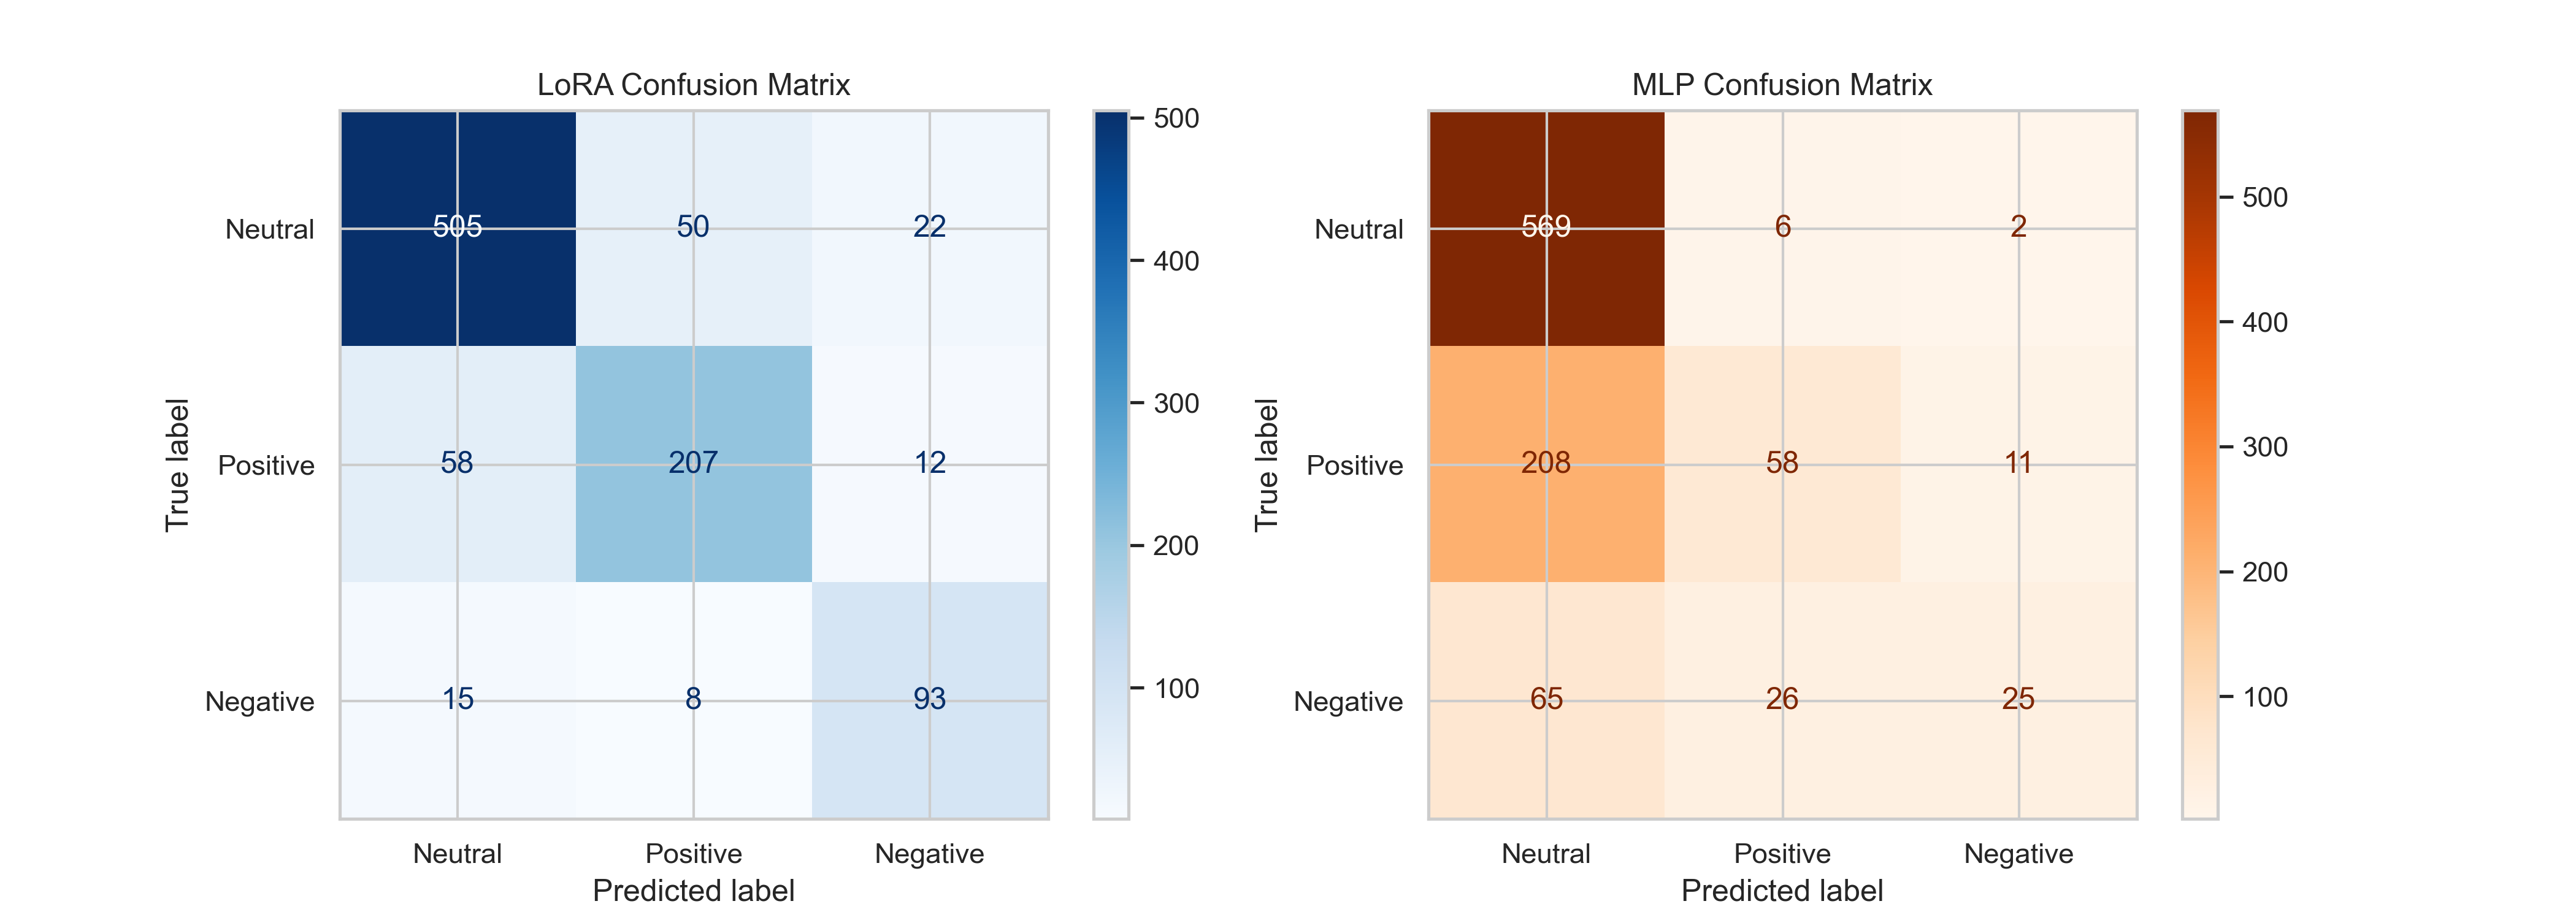
\includegraphics[width=0.8\textwidth]{../fig/confusion_matrices_comparison.png}
    \caption{Confusion Matrices}
\end{figure}
% 请在此处插入你的比较图片
\begin{figure}[h]
\centering
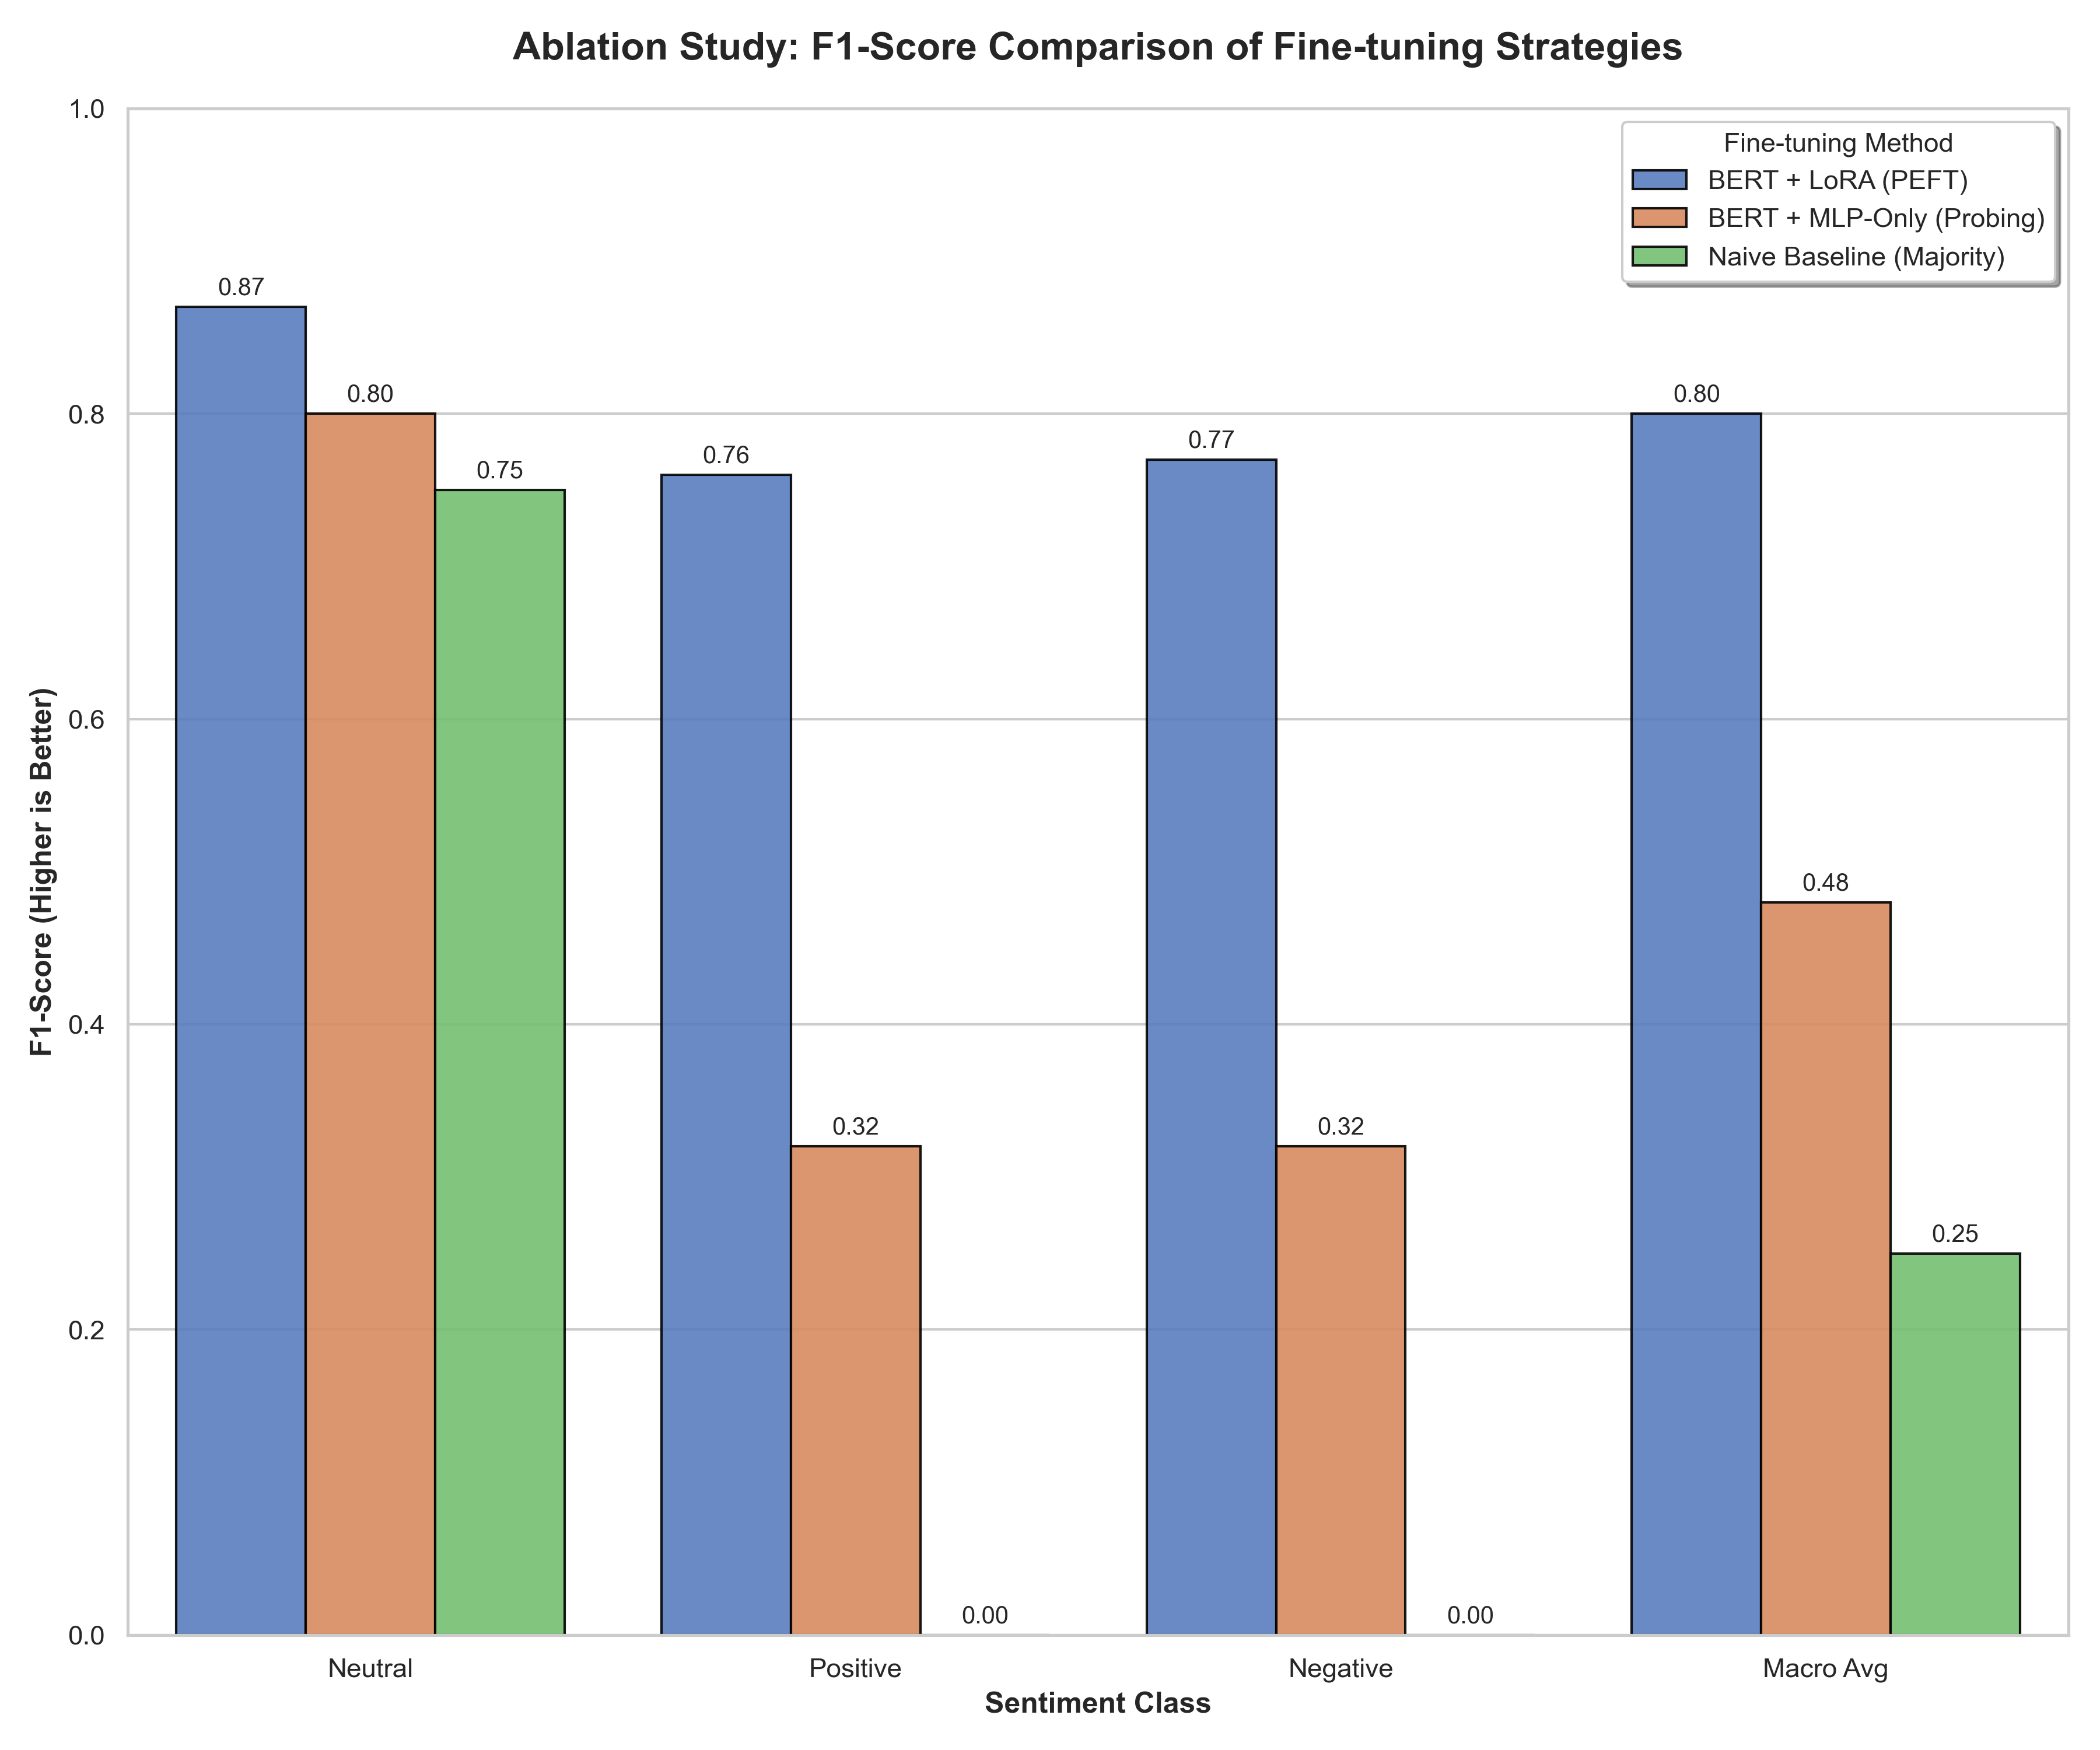
\includegraphics[width=0.6\textwidth]{../fig/ablation_study_f1_comparison.png}
\caption{Comparison Between Models}
\end{figure}
It is obvious that the fine tuning optimize the performance of model significantly, with little computation resource consumed. 
\subsection{Analysis}
The substantial performance gap between \textbf{Linear Probing} (F1: 0.48) and \textbf{LoRA Fine-tuning} (F1: 0.80) highlights the limitations of static feature extraction. 

In the baseline scenario, the frozen BERT encoder treats financial terms with general linguistic semantics. For instance, the word \textit{"decrease"} might be encoded as a neutral movement in general text, but in a financial context like \textit{"decrease in net profit"}, it carries a strong negative polarity. By adapting the \texttt{query} and \texttt{value} projection matrices via LoRA, the model learns to \textbf{re-weight its attention}, effectively "fine-tuning" its focus toward domain-specific keywords that were previously overlooked by the general-purpose backbone.
\section{Discussion}
\subsection{Obstacles \& Solutions}
One major obstacle encountered during the initial training phase was \textbf{Loss Stagnation}. Despite the theoretical efficiency of LoRA, our early experiments yielded an F1-score of approximately \textbf{0.5}, suggesting the model was performing no better than random guessing.
Upon analyzing the training logs, we observed that the loss remained trapped around $1.0$ with negligible improvement over the first half-epoch:
\begin{quote}
    \textit{\{'loss': '1.094', 'epoch': '0.08'\} $\rightarrow$ \{'loss': '1.017', 'epoch': '0.24'\} $\rightarrow$ \{'loss': '0.970', 'epoch': '0.45'\}}
\end{quote}

The stagnation in loss, coupled with the limited update steps (only 3 epochs), indicated that the initial learning rates (LoRA: $5 \times 10^{-5}$, MLP: $3 \times 10^{-4}$) were too conservative. The weight updates were insufficient to move the low-rank adapters from their initialization toward a global minimum within the short training window.

To overcome this, we recalibrated the optimization strategy by increasing the learning rates to \textbf{$2 \times 10^{-4}$ for LoRA} and \textbf{$2 \times 10^{-3}$ for the MLP head}. This more aggressive approach provided the necessary "gradient push" for the small set of trainable parameters. Following this adjustment, the loss showed a consistent downward trend, and the F1-score successfully converged to its peak value, validating that parameter-efficient methods often require higher learning rates than traditional fine-tuning.
\subsection{Future Directions}
Implementing Retrieval-Augmented Generation to provide the model with real-time market context (e.g., 2026 Q1 GDP data) to further reduce hallucinations in sentiment boundary cases.
\newpage
\section{Appendix}
\subsection{data\_loader.py}
\begin{figure}[H]
    \centering
    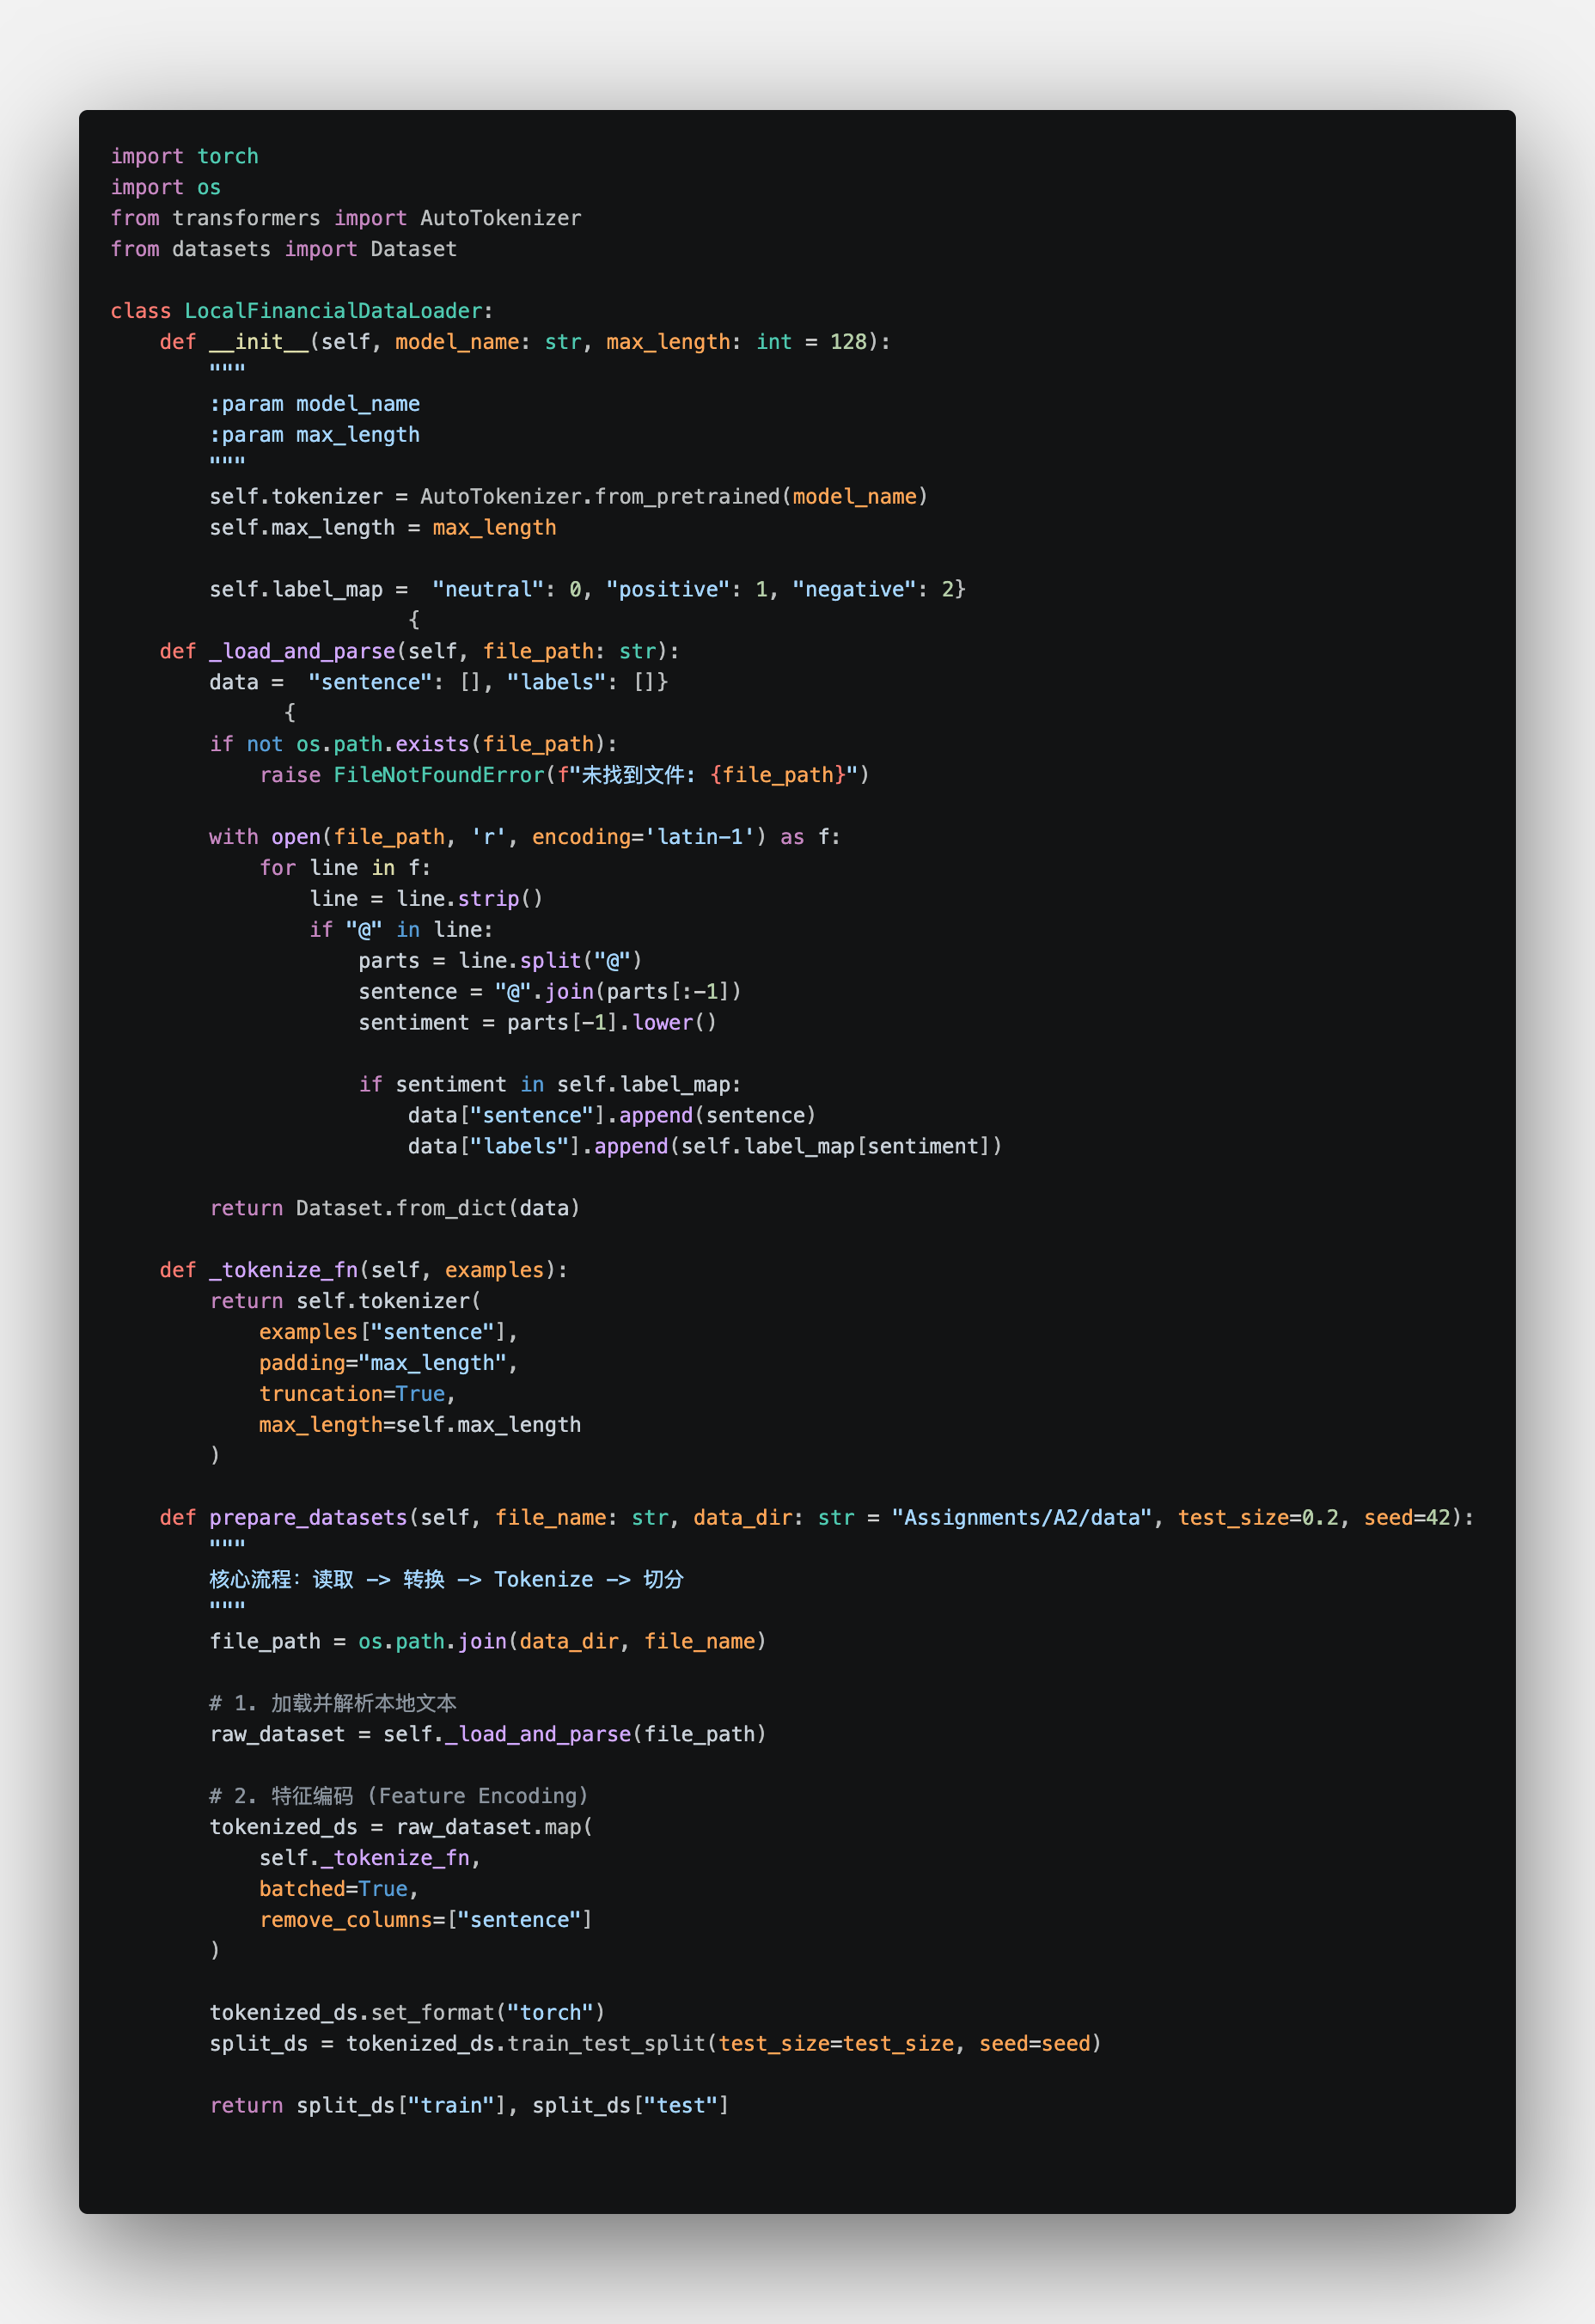
\includegraphics[width=0.7\textwidth]{../fig/data_loader.png}
\end{figure}
\newpage
\subsection{model\_lib.py}
\begin{figure}[H]
    \centering
    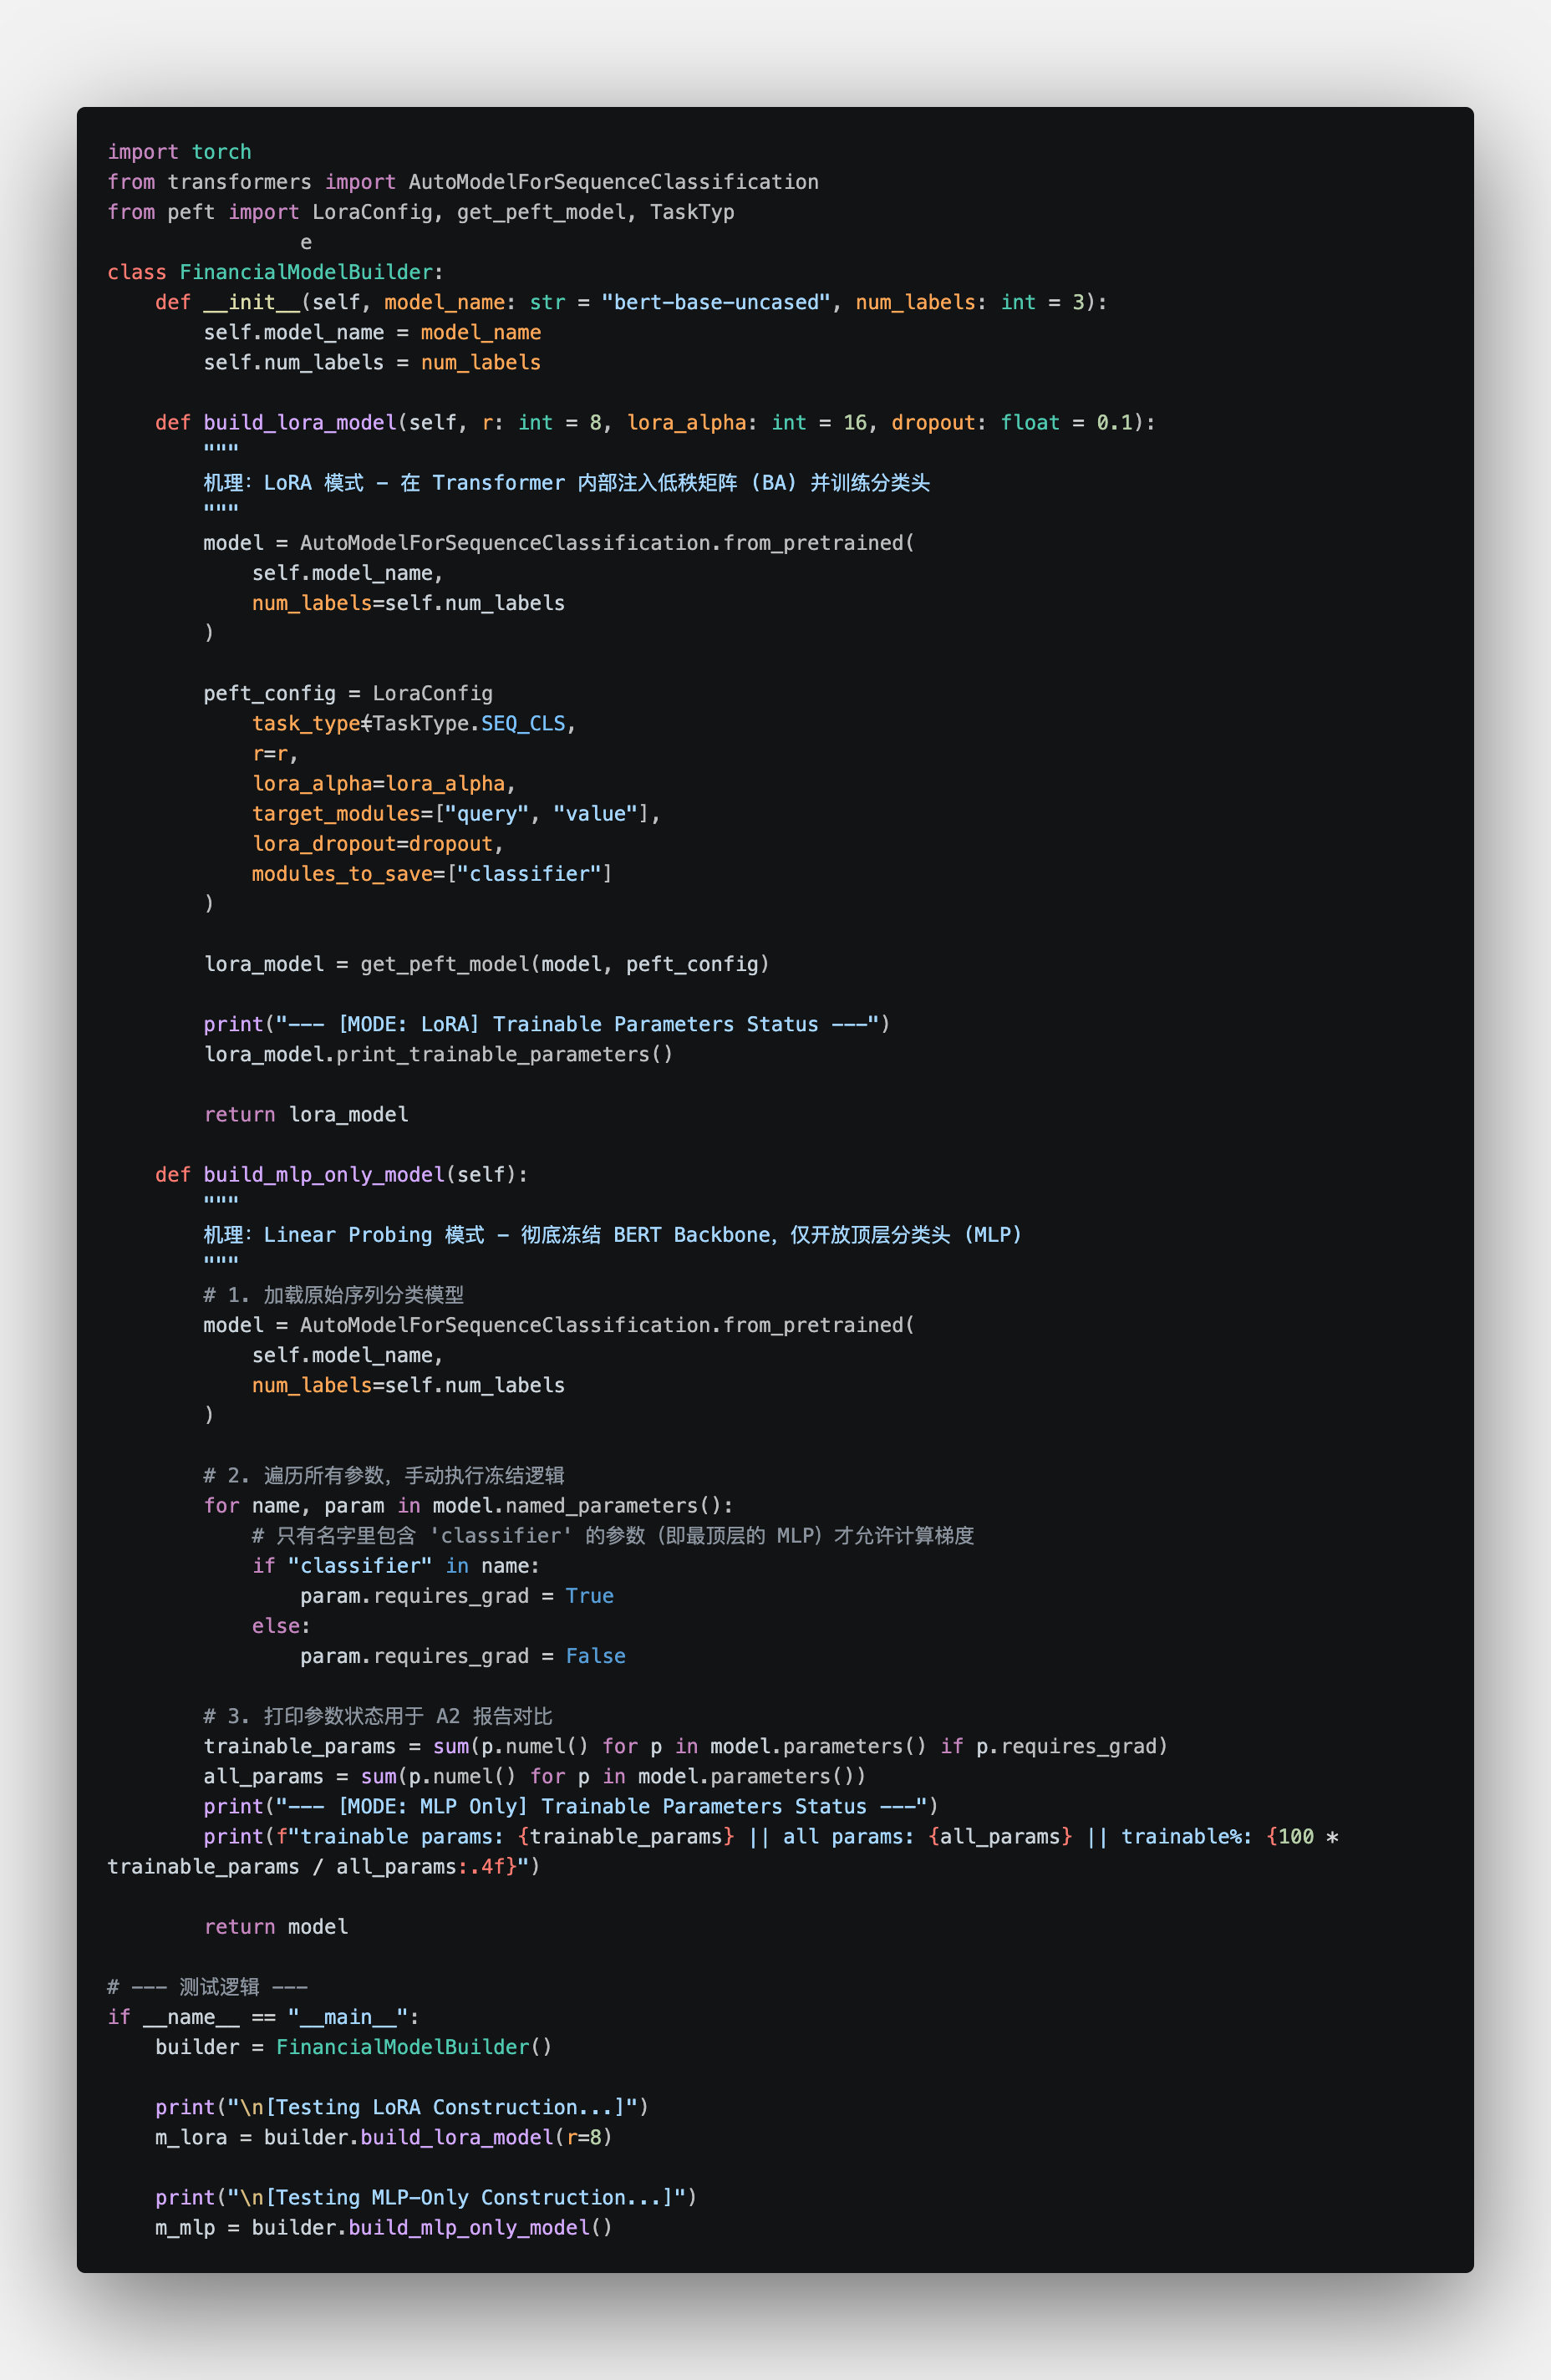
\includegraphics[width=0.7\textwidth]{../fig/model_lib.png}
\end{figure}
\newpage
\subsection{train.py}
\begin{figure}[H]
    \centering
    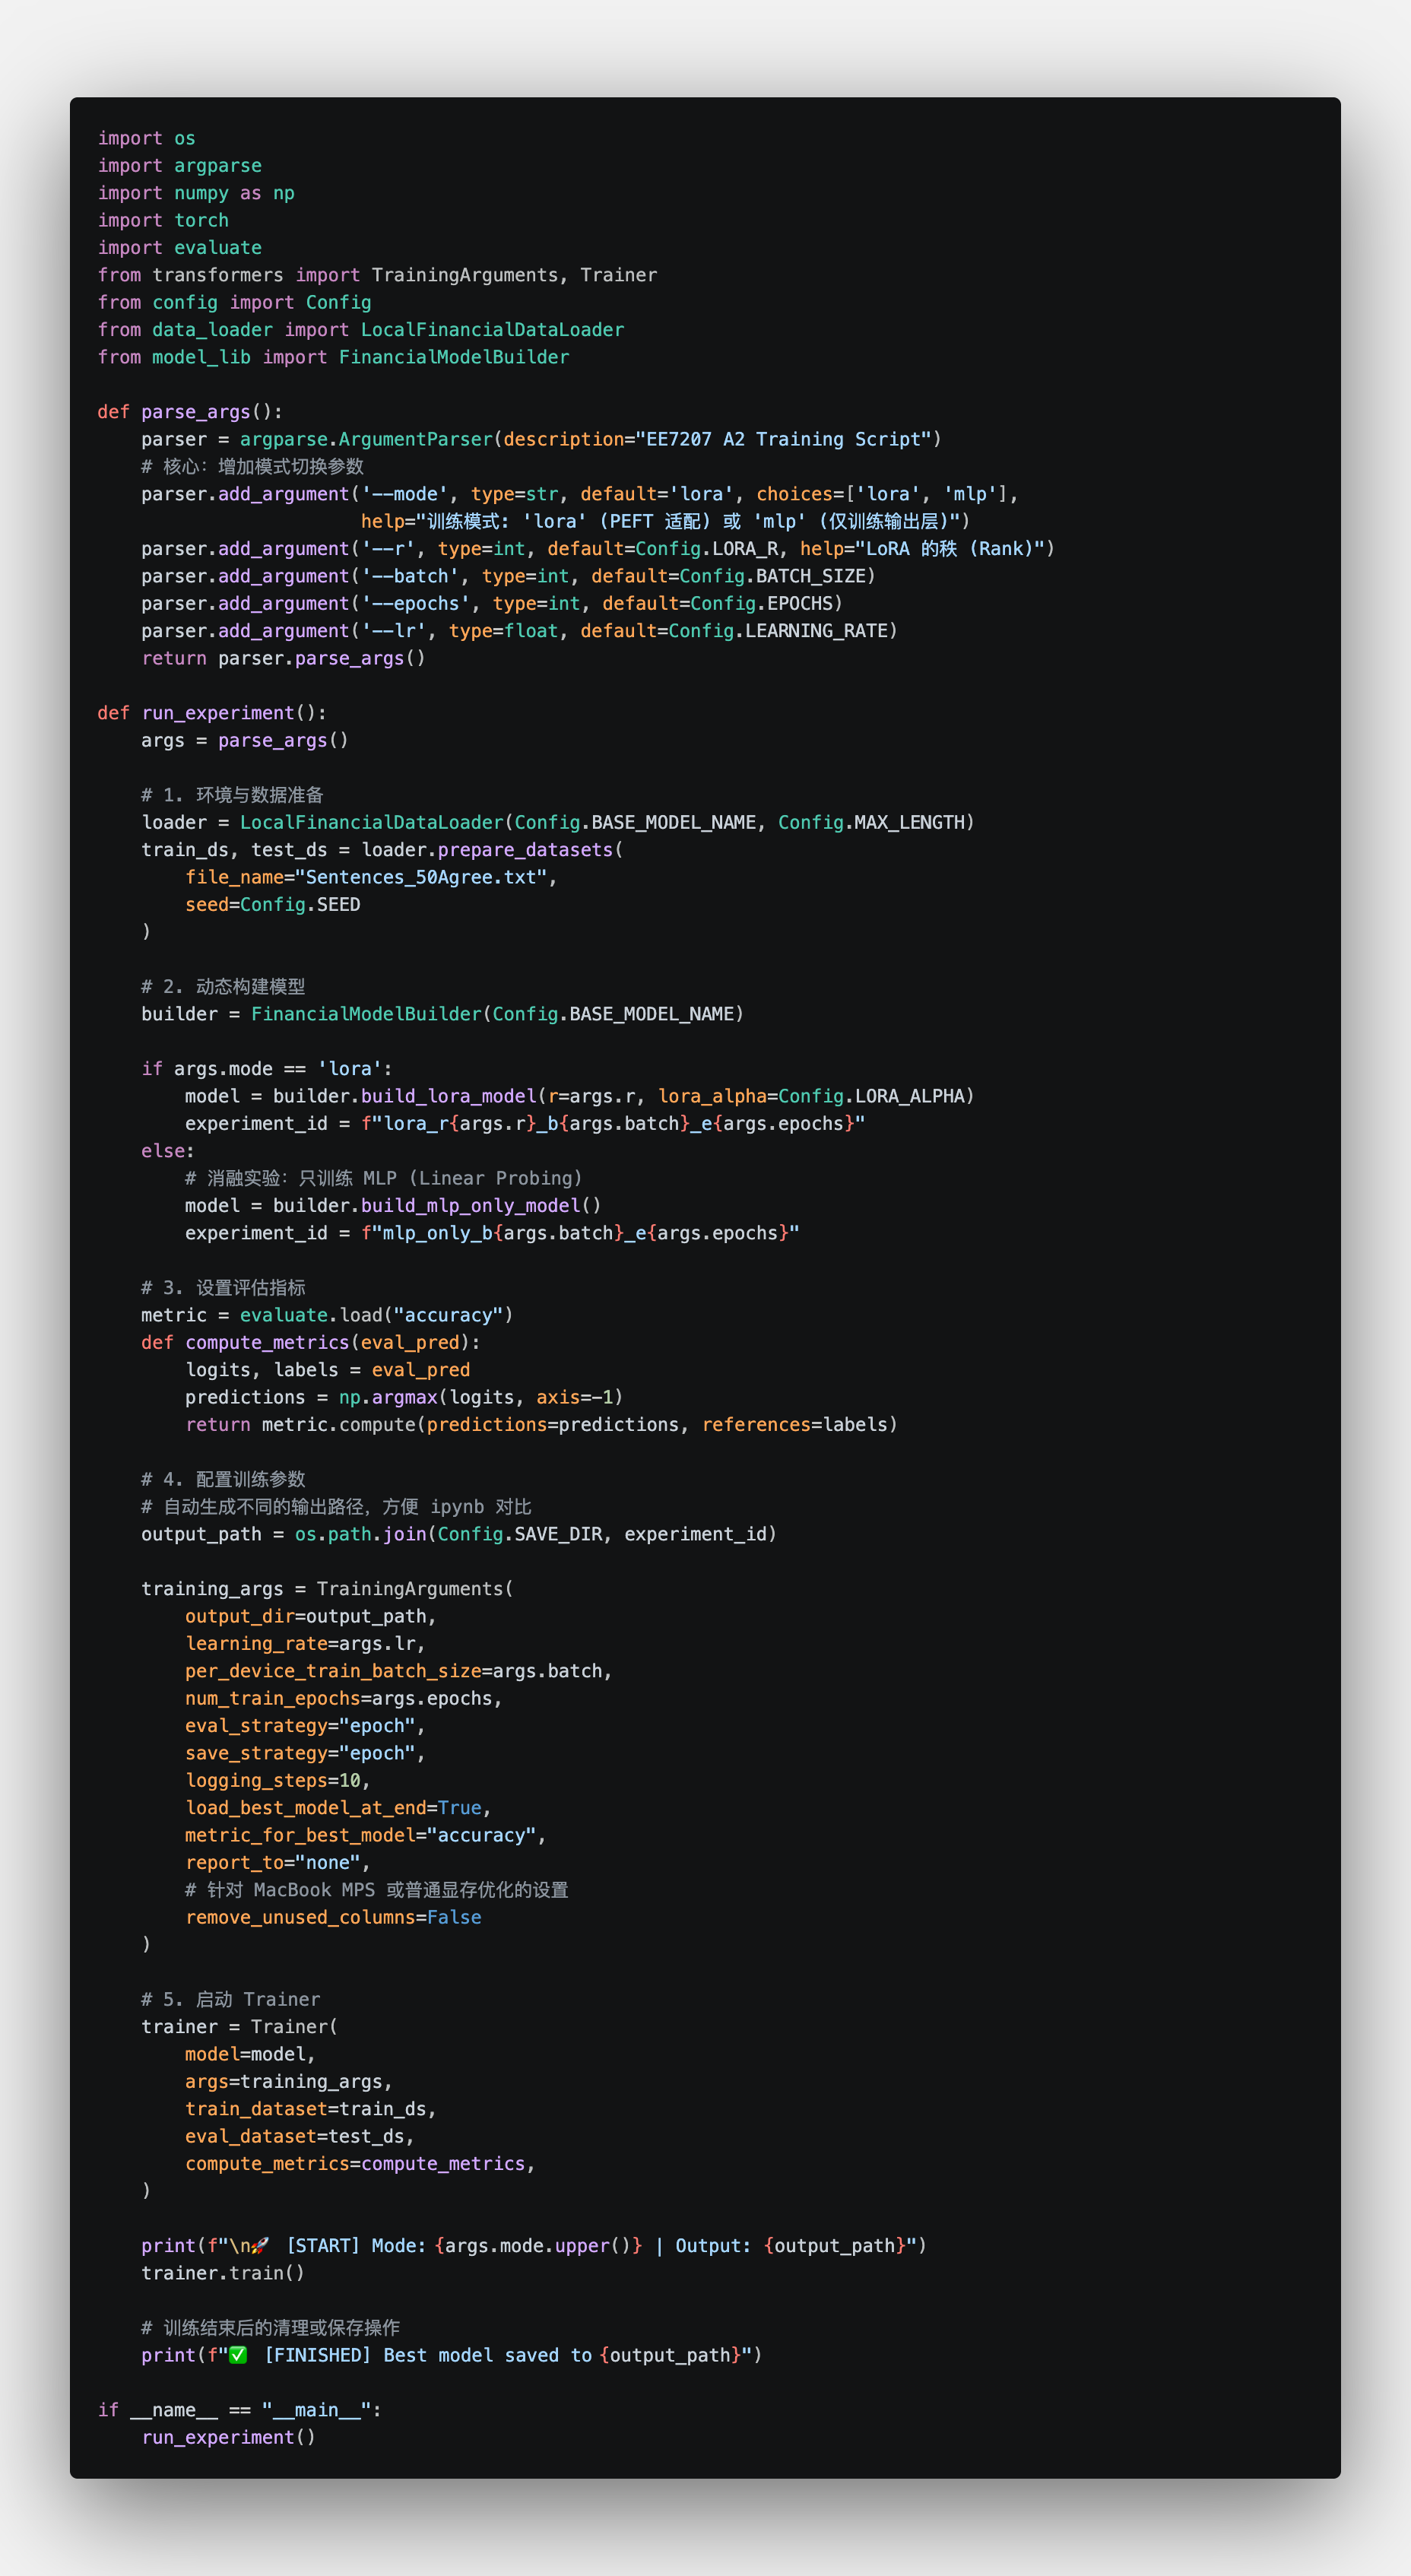
\includegraphics[width=0.7\textwidth]{../fig/train.png}
\end{figure}
\newpage
\subsection{inference.py}
\begin{figure}[H]
    \centering
    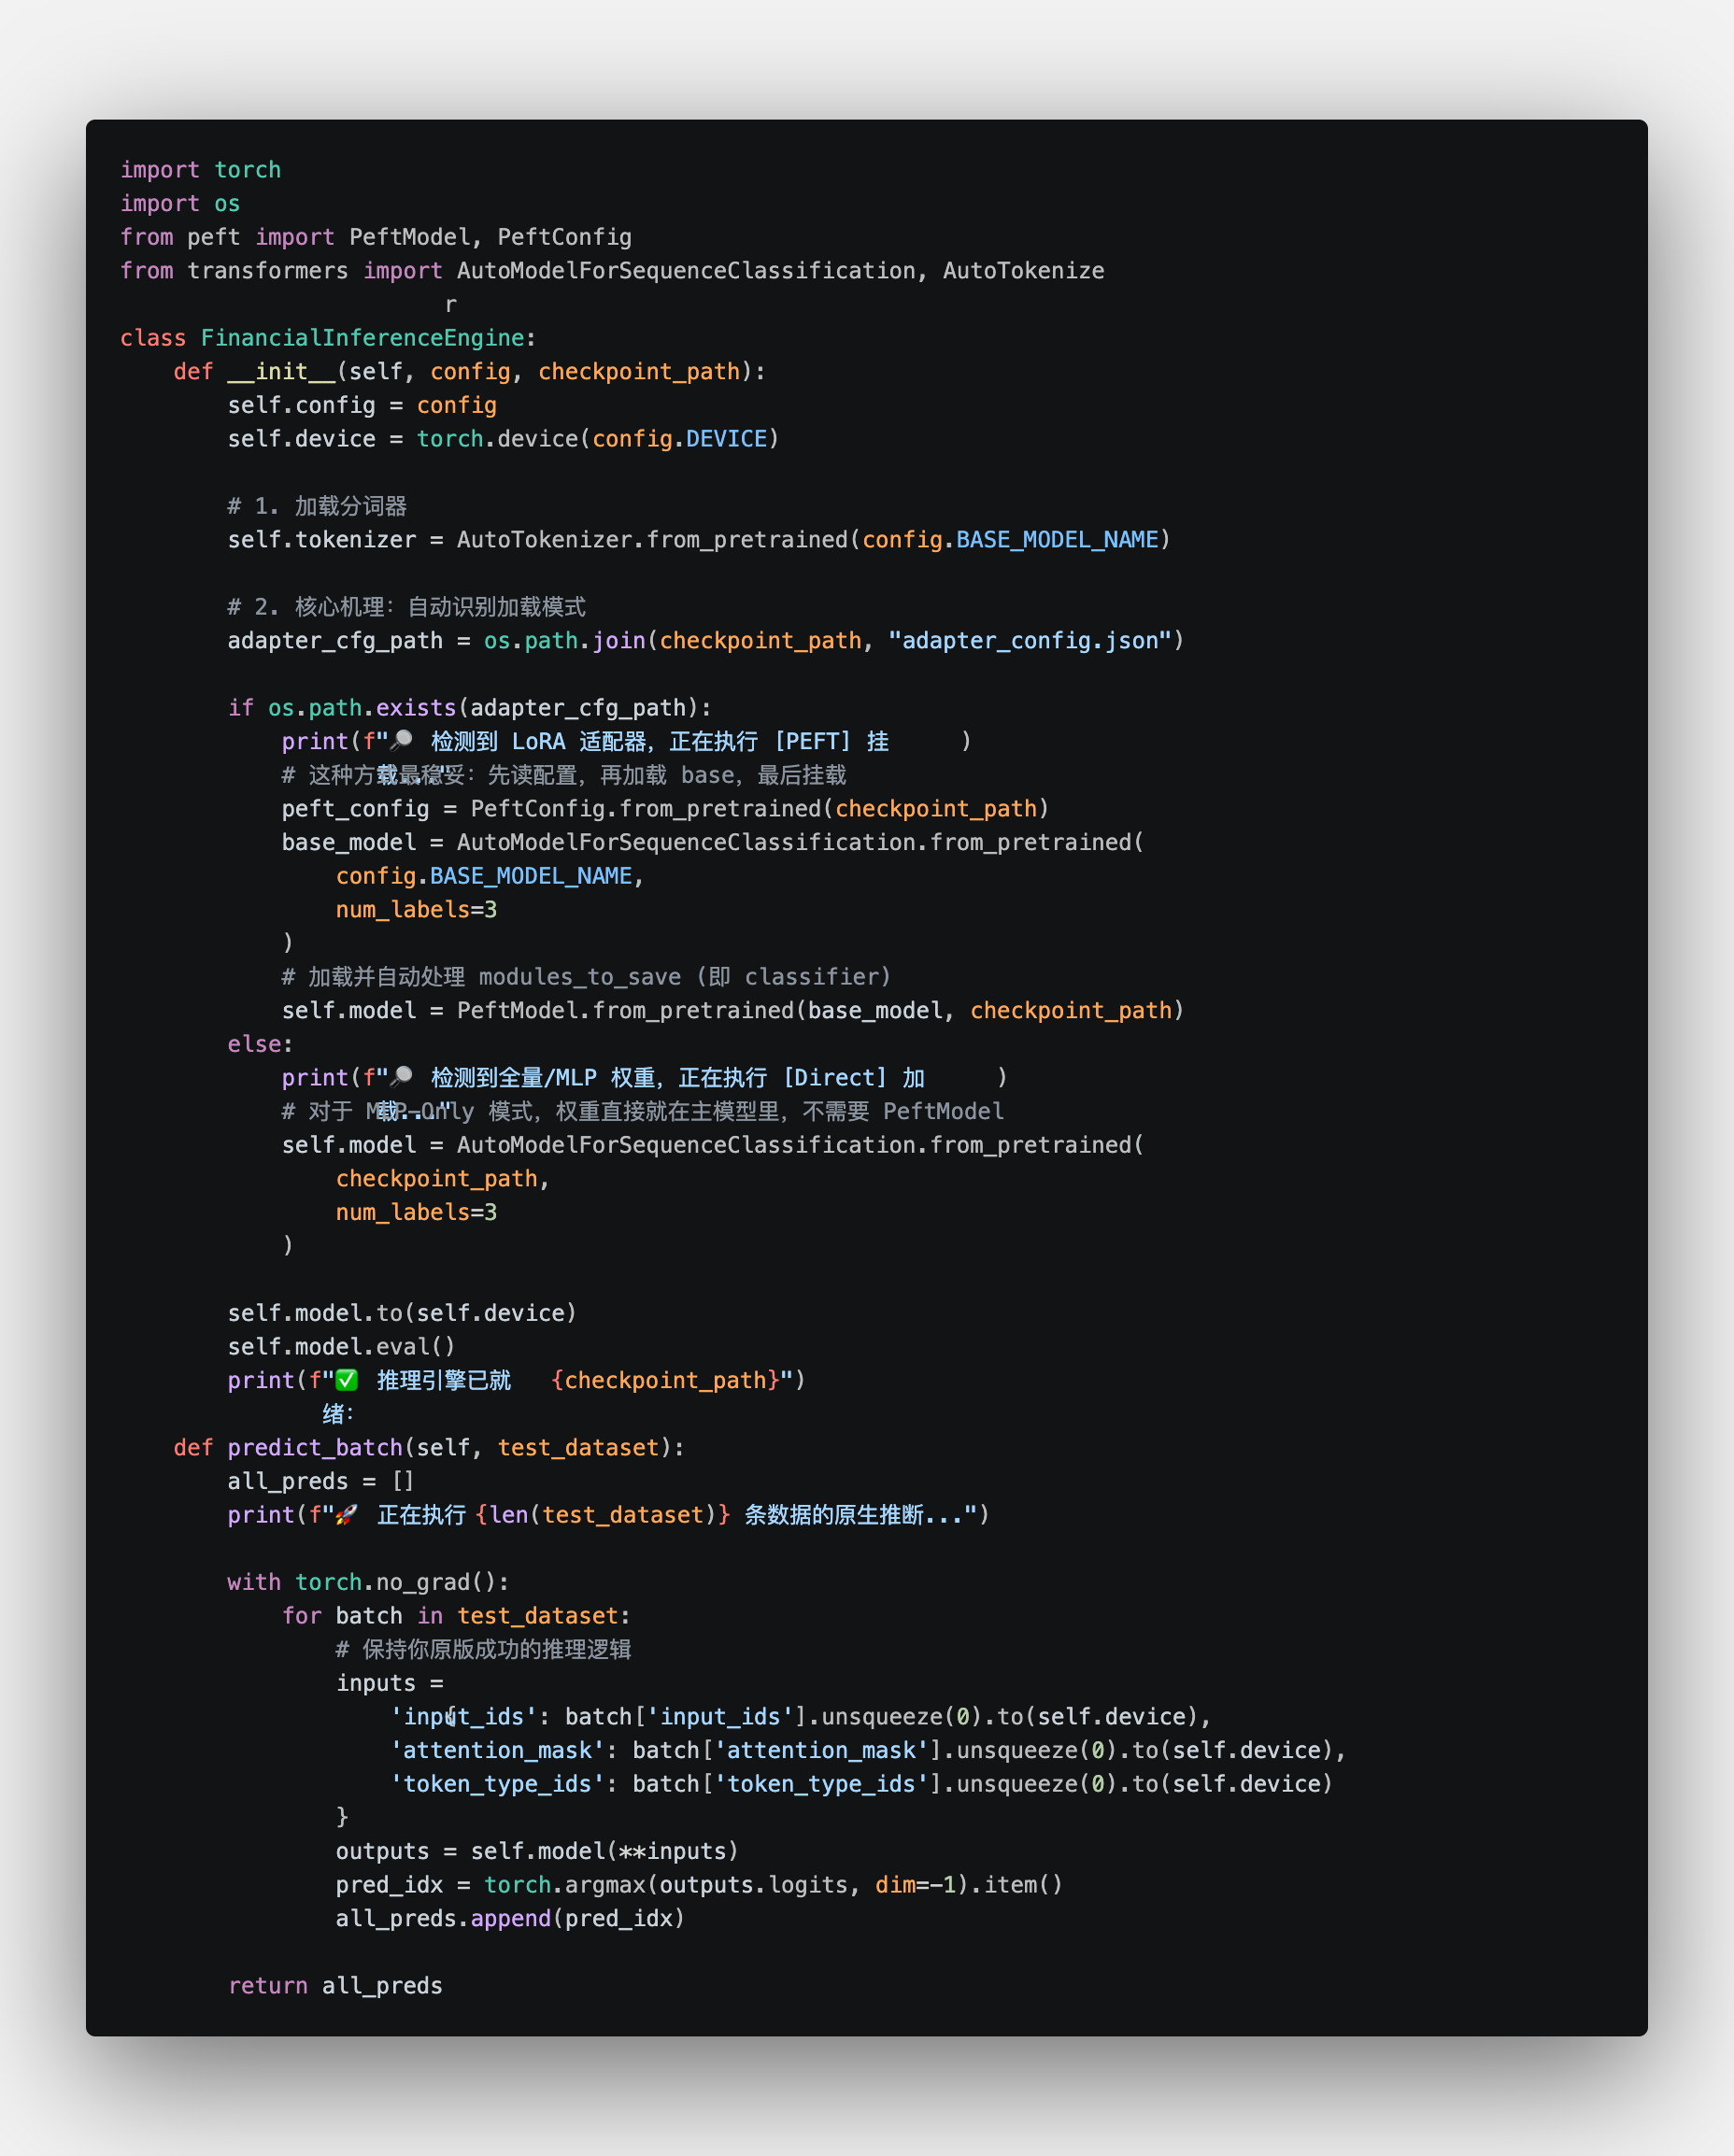
\includegraphics[width=0.7\textwidth]{../fig/inference.png}
\end{figure}
\end{document}